\clearpage

\def\chaptertitle{System Implementation}

\lhead{\emph{\chaptertitle}}

\chapter{\chaptertitle}
\label{ch:experimental-setup}

In this chapter, we will first discuss the underlying hardware and assumptions used in creating the experiments in section \ref{sec:ch4-hardware-assumptions}. Section \ref{sec:ch4-microservice-overview} will then describe the microservice application used to test the algorithm, along with the method used to generate data. Finally, we will discuss the proposed algorithm itself, and how each subsection of the autoscaler interacts with Kubernetes.

\section{Microservice Overview}
\label{sec:ch4-microservice-overview}

DeathStarBench \footnote{\url{https://github.com/delimitrou/DeathStarBench/tree/master/socialNetwork}}, a social media microservice developed by Y. Gan et al. \cite{gan2019open} is deployed on Kubernetes. The application mimics a large-scale social network application and supports common actions such as registering and login for user credentials, creating user posts on their timeline, reading other user timelines, receiving follower recommendations, following and unfollowing of other users, and searching for users or posts. Figure \ref{fig:social} shows the architecture of the micro-service.\par

The end-to-end service implementation depicts a social network with a broadcast style approach. The user or client sends requests using HTTP to the front-end layer. These requests are processed using a load balancer implemented using an open-source deployment known as NGINX \footnote{\url{https://nginx.org/en/}}. NGINX then specifies the web server that has been selected, and talks to the microservices in the logic layer, which are responsible for composing and displaying the user and timeline posts. The logic layer also consists of microservices for serving advertisements, search engines, and other capabilities commonly found in large scale applications. The search and advertisement engines are machine learning plugins capable of serving recommendations based on user interactions. The logic layer is capable of handling posts containing text, links, and media. Users can also mark other user's posts as favourites, re-post them, and reply to them privately or publicly. Users can also follow, unfollow, or block others. All these interaction results are stored in the storage layer, which uses memcached for caching results, and MongoDB for sotring user profiles, posts, media, and recommendations in a persistent manner.

Users can sign in to the application website by connecting to the user interface deployment, which can be assigned a DNS address. For experimental purposes, we simply use the Kubernetes node IP address and the social media application port. For example, an API request for reading user timelines will look as follows:\par

http://<node-IP>:<app-port>/wrk2-api/user-timeline/read

\begin{figure}[htb]
    \centering
    \caption{DeathStarBench Social-Network Architecture, courtesy Y. Gan et al. \cite{gan2019open}}
    \label{fig:social}
    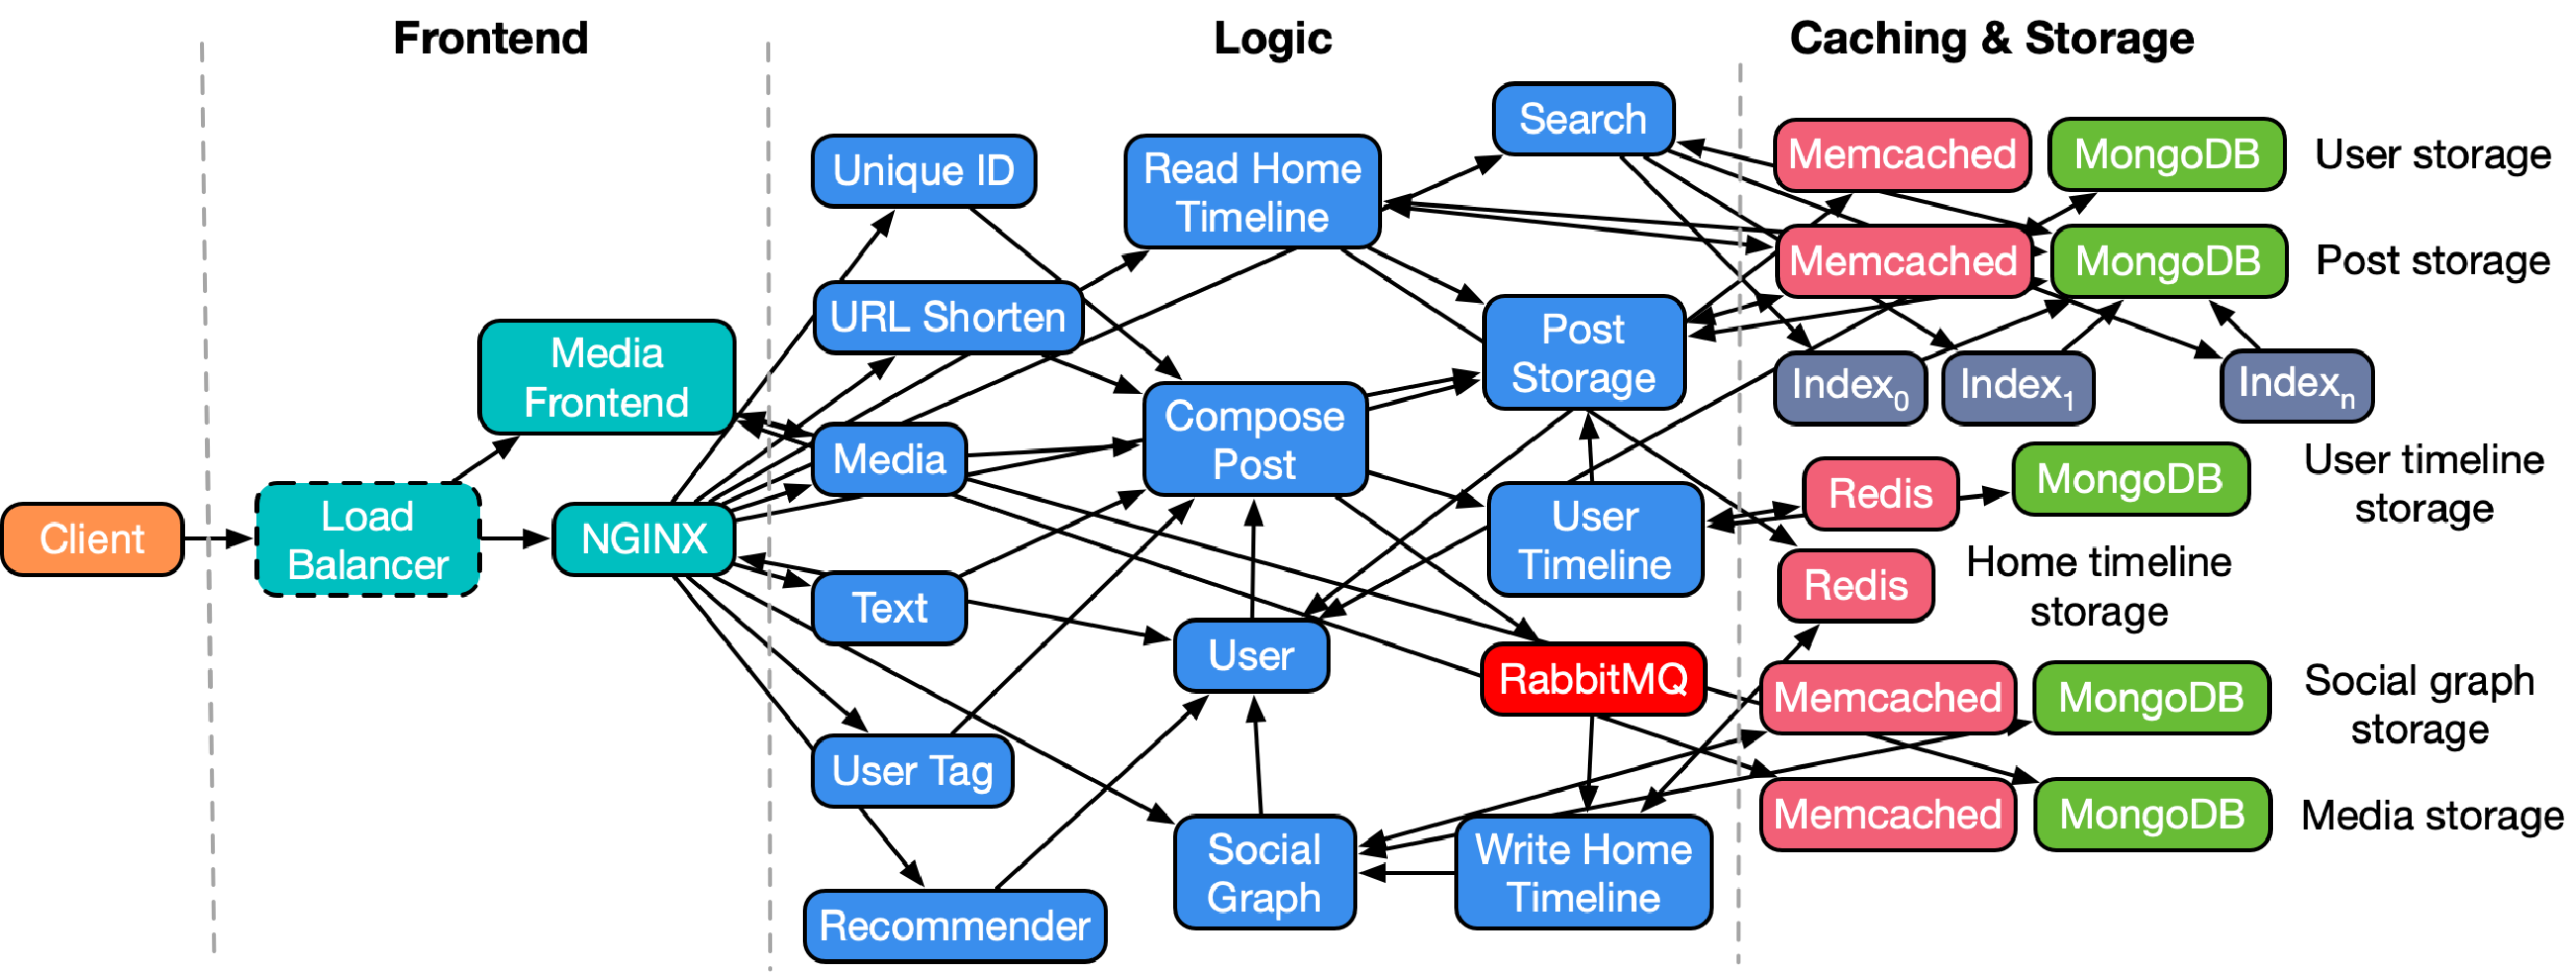
\includegraphics[width=1.0\linewidth]{Figures/Social-Network-Architecture.pdf}
\end{figure}

\section{Data Generation}
\label{sec:data-generation}

The social media deployment also comes with an HTTP workload generator, which
is leveraged to create a realistic simulation of a typical day of workload for the microservice application. The generator, known as ``wrk2'', is an open-loop load generator. HTTP requests are sent out according to the user configuration, regardless of whether or not the responses of the previous requests have been received. This avoids issues such as queuing delays in the server. The workload generator supports a variety of load generation use-cases, as well as different APIs. For example, a POST request a total load generation of 8 requests per second using 2 threads, with 5 open HTTP connections, and for a duration of 30 seconds looks like:\par

\begin{lstlisting}[
  caption={Workload generation example},
  captionpos=t,
  label={lst:workload-gen-example},
  language=bash
]
$ wrk2 -t2 -c5 -d30s -R8 http://<node-IP>:<app-port>/wrk2-api/post/compose
\end{lstlisting}

A typical IoT application in the edge has a semi-predictable workload pattern. In this experiment, it is assumed that the workload peaks in the morning and evening, while seeing moderate usage during the afternoon. The workload is lowest at night. The workload simulator was modified to introduce an element of randomness to mimic realistic weekly workloads, which can vary on occasions such as weekends and public holidays.\par

To achieve this, an IoT workload algorithm was created for leveraging the wrk2 generator to achieve this time-series. This is explained in algorithm \ref{alg:work-gen}. A constant workload is set for night time, while different workloads for different day time hours are set. The algorithm also contains a small random ``offset'' variable to depict the randomness inherent in the workload. This workload is then executed using the wrk2 generator to apply the HTTP load on the microservice.

%TC:ignore
\begin{algorithm}
    \caption{IoT workload generation algorithm}
    \label{alg:work-gen}
    \begin{algorithmic}
        \State $offset \gets \alpha$
        \State $night\_workload \gets \omega$
        \State $day\_workload \gets [ \delta_1, \delta_2, ... , \delta_{18}]$
        \While{True}
            \For {i $\leftarrow$ 0 ... 6}
                \State $result \gets generate(night\_workload + \mathcal{U}(-offset,offset)$
            \EndFor
            \For {i $\leftarrow$ 0 ... 18}
                \State $result \gets generate(day\_workload[i] + \mathcal{U}(-offset,offset)$
            \EndFor
        \EndWhile
    \end{algorithmic}
\end{algorithm}
%TC:endignore

\section{Hybrid Autoscaler Architecture}
\label{ref:hybrid-auto-arch}

\suhrid{Elaborate on this section. Put the detailed hybrid architecture diagram here and explain it before going through the individual sections. Use the text in Euro-Par paper}

In this section, the overall architecture of our proposed hybrid autoscaler will be discussed. First, a brief background of how the social media application is connected to Kubernetes, so that it can send custom metrics such as application CPU usage and latency. Then we will discuss these custom metrics further, and how they are integrated for use in the horizontal pod autoscaler.\par

With this background, we proceed with the discussion of the reactive subcomponent of the hybrid autoscaler, discussing its architecture and overall role within the algorithm. We then discuss the proactive autoscaler. This includes the components which are used to train the time-series analyzer, the choice of algorithm, and the overall goals of the forecaster. Finally, the autoscaler daemon, which controls the reactive and proactive subcomponents, as well as tunes the proactive autoscaler, will be briefly discussed.\par

\subsection{Social Media Metrics Export To Kubernetes}
\label{subsec:metrics-export}

The social media application comes bundled with Jaeger \footnote{\url{https://www.jaegertracing.io/}} deployment. Jaeger is an open-source distributed tracing platform, capable of tracking several application metrics of each network request and per-microservice request, and stores them in a centralized database. One such metric is the details of API latency for the application. The latency information is extremely detailed, and is broken down per each deployment in the social media architecture as defined by Figure \ref{fig:social}.\par

Before this information can be useful in the autoscaling solution, it must be imported to Kubernetes in a readable format. This was achieved through the use of a deployment called Prometheus. Prometheus \footnote{\url{https://prometheus.io/docs/introduction/overview/}} is an open-source deployment used for monitoring applications. Prometheus consists of a multi-dimensional data model for storing time-series data through key/value pairs, a custom built querying language known as PromQL, which is used to leverage and search through this data model, and a graphing and dashboard user interface to aid in visualization.\par

To facilitate the export of Jaeger metrics to Prometheus, a custom deployment was created which scrapes these metrics at a given time interval, and pushes it to Prometheus. The ``Jaeger-Scraper'' deployment was a JavaScript express server using the open-source prometheus-client library, and the server code was as follows:

%TC:ignore
\begin{lstlisting}[
  caption={Jaeger-Scraper server},
  captionpos=t,
  label={lst:jaeger-scraper},
  float=ht
]
const avg_counter = new Gauge({
        name: 'wrk2_avg_api_latency',
        help: 'Jaeger average post API latency (ms)'
});

get('/metrics', async (req, res) => {
    let url = process.env.JAEGER_URL;
    const data = await axios.get(url);
    let avg_duration = 0;

    let durations = data.map(api => {
        let duration = api.spans.find(
            span => span.references.length === 0
        );
        return duration;
    });

    avg_duration = durations.reduce( (a,b) => a+b ) / durations.length;
    avg_counter.set(avg_duration);

    res.set('Content-Type', avg_counter);
});
\end{lstlisting}
%TC:endignore

Once this server is deployed on the Kubernetes cloud layer, a service-monitor for Prometheus is written, which tells Prometheus to invoke the GET API this server exposes at a set interval of time. For this thesis, this interval was set at 15 seconds.

%TC:ignore
\begin{lstlisting}[
  caption={Jaeger-Scraper service monitor},
  captionpos=t,
  label={lst:jaeger-scraper svc-monitor},
  float=ht
]
apiVersion: monitoring.coreos.com/v1
kind: ServiceMonitor
metadata:
  labels:
    app: jaeger-scraper
  name: jaeger-scraper-svc-monitor
spec:
  endpoints:
  - interval: 15s
    port: http
  selector:
    matchLabels:
      app: jaeger-scraper
\end{lstlisting}
%TC:endignore

Listing \ref{lst:jaeger-scraper-metric} below shows an example of how the metrics are displayed. With the latency metrics now present in Prometheus, the next step to importing these metrics to the custom metrics server was deployed.\par

%TC:ignore
\begin{lstlisting}[
  caption={Jaeger-Scraper metrics collector},
  captionpos=t,
  label={lst:jaeger-scraper-metric},
  float=ht
]
$ curl $(kubectl get service jaeger-scraper --template \
'{{.spec.clusterIP}}'):8081/metrics
# HELP wrk2_avg_api_latency Jaeger average post API latency (ms)
# TYPE wrk2_avg_api_latency gauge
wrk2_avg_api_latency 0
\end{lstlisting}
%TC:endignore

By default, Kubernetes autoscaling can scale resources based on CPU and memory utilization. However, for more complex use-cases, more metrics need to be taken into account to make such decisions. To aid in this process, the Prometheus Adapter \footnote{\url{https://github.com/kubernetes-sigs/prometheus-adapter}} was created to leverage the metrics collected and stored by the Prometheus deployment, and feed them to Kubernetes. These metrics are exposed via an API service and are consumed by the hybrid autoscaler for decision making.\par

The prometheus adapter requires a configuration map (ConfigMap) to translate Prometheus metrics to Kubernetes custom metrics. The adapter does so in four steps.

\begin{itemize}
    \item Discovery - The adapter discovers the metrics available in Prometheus
    \item Association - Figure out the association between each metric and Kubernetes resource
    \item Naming - Assigns a name to these resources through which the custom metrics API can expose them
    \item Querying - Queries the Prometheus deployment to get the actual metric numbers
\end{itemize}

The hybrid autoscaler requires the default CPU metric, as well as the custom latency metric. Thus we define these this additional metric for configuring in Kubernetes. Listing \ref{lst:prometheus-adapter-configmap} shows the discovery, association, naming, and querying steps to do so.

%TC:ignore
\begin{lstlisting}[
  caption={Prometheus adapter configmap},
  captionpos=t,
  label={lst:prometheus-adapter-configmap},
  float=ht
]
apiVersion: v1
kind: ConfigMap
metadata:
  name: custom-metrics-prometheus-adapter
data:
  config.yaml: |
    rules:
    - metricsQuery: <<.Series>>
      name:
        as: ${1}_per_minute
        matches: ^(.*)
      resources:
        template: <<.Resource>>
      seriesQuery: wrk2_avg_api_latency{namespace!=""}
\end{lstlisting}
%TC:endignore

Now, the Kubernetes custom metrics API exposes the following additional APIs in listing \ref{lst:custom-metrics-example}

%TC:ignore
\begin{lstlisting}[
  caption={Custom metrics API example},
  captionpos=t,
  label={lst:custom-metrics-example},
  float=ht
]
$ kubectl get --raw /apis/custom.metrics.k8s.io/v1beta1 | jq .
{
  "groupVersion": "custom.metrics.k8s.io/v1beta1",
  "resources": [
    {
      "name": "services/wrk2_avg_api_latency_per_minute",
      ...
    },
    {
      "name": "pods/wrk2_avg_api_latency_per_minute",
      ...
    },
    {
      "name": "namespaces/wrk2_avg_api_latency_per_minute",
      ...
    }
  ]
}

$ kubectl get --raw \
/apis/custom.metrics.k8s.io/v1beta1/namespaces/default\
/services/*/wrk2_avg_api_latency_per_minute | jq .
{
  "kind": "MetricValueList",
  "apiVersion": "custom.metrics.k8s.io/v1beta1",
  "items": [
    {
      "describedObject": {
        "kind": "Service",
        ...
      },
      "metricName": "wrk2_avg_api_latency_per_minute",
      "value": "0"
    }
  ]
}


\end{lstlisting}
%TC:endignore

\subsection{Reactive Autoscaler}
\label{subsec:reactive-auto-subsection}

With the custom metrics now being exposed by Kubernetes, all the tools required for the reactive autoscaling sub-component are in place. This will be built as an extension of the default Kubernetes default horizontal pod autoscaler.\par

At a high-leve, the default Kubernetes autoscaler operates on the ratio between the current and desired metric values, which can be written as:

\[ replicas_{desired} = \lceil replicas_{current} \times \frac{metric_{current}}{metric_{desired}}\rceil\]

For example, if the desired value is 50 resource units, the current value is 100, and the number of current replicas is 1 then the number of desired replicas will be $\lceil 1 \times \frac{100}{50}\rceil = 2$. There are three other important parameters which are important for reactive scaling, namely tolerance, scale up cooldown, and scaledown cooldown.\par

The tolerance is a constant which informs the Kubernetes autoscaler to skip calculating new replicas. The tolerance ratio, can be calculated as:

\[ tolerance = \abs{ \frac{metric_{current} - metric_{desired}}{metric_{current}} }\]

By default, if the tolerance value is below 0.1, autoscaling is skipped for that control loop.\par

The scale up and scale down cooldowns control how quickly autoscaling occurs. The default approach which is set by Kubernetes can be concisely stated as ``Scale up as quickly as possible, while scale down very gradually''. Therefore, the default scale up cooldown is set to 0 seconds, meaning that the moment the desired replica value increases, the autoscaling will be initiated. However, the default cooldown is set to 300 seconds, meaning that if the desired replica value is decreased, it must remain decreased for 300 seconds (or 20 control loops) before the resources are scaled down.\par

The reactive autoscaler will customize the default autoscaler by setting both the cooldown values to 15 seconds, or one control loop. This ensures that reactive autoscaling occurs as quickly as possible, to minimize SLA violations, while decreasing the chances of resources constantly being scaled up and down in a yo-yo manner \cite{sides2015yo}. Listing \ref{lst:reactive-cooldown-config} shows the configuration changes to achieve this.\par

%TC:ignore
\begin{lstlisting}[
  caption={Reactive autoscaler cooldown configuration},
  captionpos=t,
  label={lst:reactive-cooldown-config},
  float=ht
]
spec:
  behavior:
    scaleDown:
      policies:
      - periodSeconds: 15
        type: Pods
      stabilizationWindowSeconds: 15
    scaleUp:
      policies:
      - periodSeconds: 15
        type: Pods
      stabilizationWindowSeconds: 15
\end{lstlisting}
%TC:endignore

While these parameters are configurable by other users, experimental results showed that for SLA-compliant applications, these parameters were able to produce the best results for a wide array of use-cases.

\subsection{Proactive Autoscaler}
\label{subsec:proactive-auto-subsection}

The proactive autoscaler has a Kubernetes configuration that is similar to the reactive one. The same cooldown values of 15 seconds are applied here as well, to keep it consistent with the reactive solution.\par

For autoscaling proactively, a custom metric $forecasted_cpu$ which defines the future cpu workload expected to be exerted on the social media application $\mathcal{T}$ seconds in the future, where $\mathcal{T}$ can be configured by the user. This $forecasted_cpu$ value will be sent to Prometheus by the forecaster. To capture this metric in the custom API, the Prometheus Adapter configuration map is modified to add the values shown in listing \ref{lst:prometheus-adapter-configmap-proactive}.

%TC:ignore
\begin{lstlisting}[
  caption={Prometheus adapter configmap},
  captionpos=t,
  label={lst:prometheus-adapter-configmap-proactive},
  float=ht
]
- metricsQuery: <<.Series>>
  name:
    as: ${1}_per_minute
    matches: ^(.*)
  resources:
    template: <<.Resource>>
  seriesQuery: forecasted_cpu{namespace!=""}
\end{lstlisting}
%TC:endignore

The forecaster portion of the autoscaler generates this metric. Several time series forecaster algorithms exist, with the two prominent ones being the more modern deep learning algorithm LSTM, and the traditional deep learning algorithm ARIMA. Siami-Namini et al. \cite{siami2018comparison} demonstrated that LSTM implementations outperformed ARIMA, reducing error rates by over 80\%. Furthermore, they were able to demonstrate that the number of deep learning ``epochs'', or the total amount of training time required for LSTM did not need to be set to a high value. In fact, setting an unreasonably high value was shown to degrade performance due to over-fitting. The authors posited that LSTM worked so well due to the ``rolling updates'' being performed on the model. The LSTM weights are only set once when the forecaster is deployed, after which they are always updated on every call of the training algorithm\par

\begin{figure}[htb]
    \centering
    \caption{Pre-processing of data, courtesy of Christopher Boucher \cite{comsolcurvefitting}}
    \label{fig:data-pre-process}
    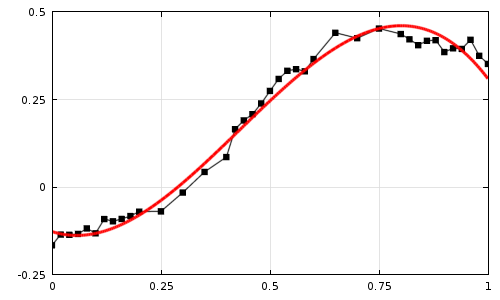
\includegraphics[width=0.6\linewidth]{Figures/Data-Pre-Processing.png}
\end{figure}

To speed up the forecast process even further and reduce the resource and time requirements, the time-series data can be pre-processed to smoothen it. Doing so makes it easier for the deep learning model to extract patterns, and reduces the training and validation loss. Figure \ref{fig:data-pre-process} shows a graph containing raw input (shown in black), and a smoothened data curve (shown in red). While the red curve contains all the requisite information of the data (such as slope of the curve, maximum and minimum value, etc.), it removes the noise, reducing the overall loss, and reducing the length of the lookback LSTM needs to perform to accurately predict future data.\par

Based on the investigations above, it was determined that LSTM time-series forecasters would be ideally suited for a proactive autoscaler designed for edge computing. Algorithm \ref{alg:proactive-forecast-alg} shows the implementation of such a forecaster. As input, algorithm takes the number of data points it should lookback on to train, the number of data points to forecast, as well as the training time epochs and learning rate. The algorithm implements a control loop every $\mathcal{P}$ seconds, where it requests the latest time series data from the autoscaler daemon. It then pre-processes this data to remove the noise as shown above, and performs one iteration of training using the configured parameters. It then computes the validation loss when doing so, and accepts this model as the ideal one if it has lower validation loss than the previous iteration, otherwise rejecting the model and using the older one instead. Finally, the model predicts the future forecasts and stores them for later use.\par

%TC:ignore
\begin{algorithm}
    \caption{Proactive forecaster algorithm}
    \label{alg:proactive-forecast-alg}
    \begin{algorithmic}
        \Require $L \geq 0, F \geq 0, 0 \leq E \leq 100, 0 \leq R \leq 1$
        \State $lookback \gets \mathcal{L}$
        \State $forecast \gets \mathcal{F}$
        \State $learning\_epochs \gets \mathcal{E}$
        \State $learning\_rate \gets \mathcal{R}$
        \State $lstm\_model \gets lstm.initialize()$
        \State $result \gets \varnothing$
        \While{$time\_series\_data \gets daemon.get\_data()$}
            \State $lstm\_input \gets get\_input(time\_series\_data, lookback)$
            \State $lstm\_input \gets preprocess\_data(lstm\_input)$
            \State $new\_model \gets train(lstm\_input, learning\_epochs, learning\_rate)$
            \If{$validation\_loss(new\_model) < validation\_loss(lstm\_model)$}
                \State $lstm\_model \gets new\_model$
            \EndIf
            \State $result \gets predict(lstm\_model, lstm\_input, forecast)$
        \EndWhile
    \end{algorithmic}
\end{algorithm}
%TC:endignore

\subsection{Autoscaler Daemon}
\label{subsec:auto-daemon-subsection}

\suhrid{Talk about the heuristic algo (Take from euro-par paper), time-series storage from Prometheus, and predicted result retrieval from forecaster}